%\documentclass[journal]{IEEEtran}
%\documentclass[12pt,onecolumn]{IEEEtran}
\documentclass[UTF8]{article}
\usepackage{ctex}\comment{text}{comment}
\usepackage{geometry,graphicx,marvosym}
\usepackage{amsmath,amsthm}
\usepackage{amsfonts}
\usepackage[usenames,dvipsnames]{pstricks}
\usepackage{pst-plot,pstricks-add}
%\usepackage{graphicx,times,amsmath,amssymb,multirow,subfigure}
\usepackage{graphicx,times,amsmath,amssymb,multirow}
\usepackage{url}
\usepackage{stfloats}
\usepackage{amsfonts,rotating}
\usepackage{color}
\usepackage{verbatim,multirow}
% setting dimension of the paper
\textwidth 7.0true in
\textheight 8.9 true in
\topmargin=-20pt
\headheight=6pt
\headsep=2pt
\oddsidemargin -0.3true in
\evensidemargin -0.4true in
\usepackage{amssymb}

\newtheorem{theorem}{Theorem}
\newtheorem{lemma}{Lemma}
\newtheorem{algorithm}{Algorithm}
\newtheorem{definition}{Definition}
\newtheorem{proposition}{Proposition}

\newcommand{\dtcwt}{\operatorname{DT-\mathbb{C}WT}}
\newcommand{\tpctf}{\operatorname{TP-\mathbb{C}TF}}
\newcommand{\ctf}{\operatorname{\mathbb{C}TF}}
\newcommand{\tr}[1]{\textcolor{red}{#1}}
\newcommand{\tb}[1]{\textcolor{blue}{#1}}
\newcommand{\mO}{{\mathcal{T}}}
\newcommand{\C}{\mathbb{C}}    %complex number field
\newcommand{\N}{\mathbb{N}}    %natural numbers
\newcommand{\R}{\mathbb{R}}    %real number field
\newcommand{\Z}{\mathbb{Z}}    %integers
\newcommand{\imag}{\mathrm{i}} % imaginary unit
\newcommand{\dR}{\mathbb{R}^d}
\newcommand{\dT}{\mathbb{T}^d}
\newcommand{\dZ}{\mathbb{Z}^d}
\newcommand{\dlp}[1]{l_{#1}(\mathbb{Z}^d)}
\newcommand{\td}{\boldsymbol{\delta}}  %Dirac/Kronicker sequence
\newcommand{\bp}{\begin{proof}}
	\newcommand{\ep}{\hfill  \end{proof} }
\newcommand{\be}{ \begin{equation} }
\newcommand{\ee}{ \end{equation} }
\newcommand{\dLp}[1]{L_{#1}(\mathbb{R}^d)}
\newcommand{\prm}{P}           %projection matrix
\newcommand{\wh}{\widehat}
\renewcommand{\le}{\leqslant}
\renewcommand{\ge}{\geqslant}
\newcommand{\bs}{\backslash}
\newcommand{\ol}{\overline}
\newcommand{\vk}{\mathsf{k}}
\newcommand{\la}{\langle}
\newcommand{\ra}{\rangle}
\newcommand{\tp}{\mathsf{T}}  %transpose
\newcommand{\conj}{\overline}
\newcommand{\supp}{\mathrm{supp}}
\newcommand{\setsp}{\;:\;}     %set separator
\newcommand{\sd}{\mathcal{S}}  %subdivision operator S
\newcommand{\tz}{\mathcal{T}}  %transition operator T
\newcommand{\wt}{\widetilde}
\renewcommand{\le}{\leqslant}
\renewcommand{\ge}{\geqslant}
\newcommand{\er}{\eqref}
\newcommand{\gep}{\varepsilon}
\newcommand{\eps}{\epsilon}
\newcommand{\gl}{\lambda}
\newcommand{\gL}{\Lambda}
\newcommand{\gd}{\delta}
\newcommand{\DAS}{\mathrm{DAS}}
\newcommand{\UDAS}{\mathrm{UDAS}}
\newcommand{\DHF}{\mathrm{DHF}}

\newtheorem{example}{Example}
\bibliographystyle{unsrt}
\newcommand{\xz}[1]{\textcolor{magenta}{\bf #1}}
\usepackage[colorlinks,linkcolor=blue,anchorcolor=blue,citecolor=blue]{hyperref}
\usepackage{indentfirst}
\begin{document}
\author{Henry}
\title{pMRI国内外研究进展}
\maketitle
\section{背景}
\par 磁共振成像(Magnetic Resonance Imaging,MRI)是一项无创的医学成像技术,该成像技术不仅不需要使用电离辐射,而且还可以得到分辨率和质量较高的病理图像,这些特性使得人体内一些器官结构、血管结构和其他生理特征都可以得到较好的可视化,因此MRI在临床上得到了广泛的应用。但是,MRI不同于计算机断层扫描(Computed Tomography,CT)等方法具有成像时间快的特性,该技术最大的障碍就是其数据采集时间过于缓慢,而且MRI设备一般都是比较密闭的空间,病人在接受扫描时可能因为空间过于密闭而导致的无法呼吸、幽闭恐惧症等。MRI技术的主要研究方向为缩短成像时间、提高成像质量,并行磁共振成像 \cite{deshmane2012parallel}(parallel Magnetic Resonance Imaging,pMRI)技术是提高MRI速度的主要方法之一,其使用一组线圈,通过获取具有不同空间灵敏度的欠采样的数据去加速成像速度,但是该方法主要受限于线圈灵敏度信息,因为难以获取较为准确的灵敏度信息。

\section{国内外研究现状}
\par 核磁共振成像技术主要分为两个步骤,分别是数据信号采集和图像重建,图像重建主要通过获取的欠采样的数据,重建出较为完整的图像。但是,受限于MRI设备和采样定理的缘故,采集数据耗费大量时间,得到的图像也也容易因为病人运动等原因产生伪影,因此众多学者致力于MRI快速成像重建的研究中,MRI图像重建方法主要分为三类:
\par 第一类,基于图像域的重建方法,该方法需要明确知道MRI设备中线圈灵敏度的信息,通过灵敏度信息将该问题建模为一个逆问题,通过非线性优化算法等进行解决;
\par 第二类,基于频率域($k$-空间)的重建方法,其灵敏度等信息隐式的存在于$k$-空间数据中,因此使用类似插值的方法估计$k$-空间缺失的数据;
\par 第三类,基于深度学习的重建方法,该方法通过MRI成像模型,构造出相对应的损失函数和正则化方法,建立深度网络进行训练。

\subsection{基于图像域的重建方法}
\par pMRI系统使用一组阵列线圈同时进行采集数据,线圈阵列由多个线圈组成,用于采集不同空间位置上的信息,越接近线圈的区域上信号会更强,这种不同空间位置导致的信号强弱被称为线圈的灵敏度。在通常情况下线圈的灵敏度未知,但是基于图像域的重建方法首先需要明确知道灵敏度,使得这一方向的大多数算法都受此影响,导致重建质量不佳。
\par 图像域重建算法中较为著名的是SENSitivity Encoding(SENSE)\cite{pruessmann1999sense},其在图像域中对伪影进行去除,但是依赖于精确的灵敏度,因此估计出精确的灵敏度是SENSE类方法的重要步骤。例如,在JSENSE\cite{ying2007joint}、TSENSE\cite{kellman2001adaptive}和mSENSE\cite{kreitner2006fast}中,JSENSE算法将MRI图像重建问题转化为线圈灵敏度和图像的联合估计问题,使用优化迭代算法进行交替求解;TSENSE提出了一种自适应灵敏度估计的方法,用以提高精确度。尽管可以通过估计的方法得到线圈的灵敏度信息,但是使用不够精确的灵敏度进行重建,导致重建得到的图像容易受到噪声放大、伪影等影响,此时可以使用正则化方法进行改良重建问题,使解约束在某一个空间中,得到较为稀疏的解。
\par 在SENSE类重建方法中经常使用的正则化方法有Tikhonov正则化($l_2$正则化)、全变差正则化(Total Variation, TV)、小波正则化和联合多种正则化方法等。在文\cite{ye2010computational}中提出一种快速求解TV正则化模型的算法,虽然TV正则化的方法有助于去除伪影, 但是也有可能产生阶梯状伪影,导致重建质量不佳,使得医生难以通过该重建图像进行诊断病情。Total Generalize Variation(TGV)\cite{bredies2010total}的提出可以消除TV这一系列缺点,从而提高图像质量。 Knoll等人\cite{knoll2012parallel}使用二阶TGV进行约束,减少了重建图像中的阶梯状伪影,同时也提出一种非线性重建方法进行求解。随着压缩感知(Compressed Sensing, CS)等理论的研究深入,Lustig等人发现MRI图像是较为稀疏的,如果使用适当的重建算法,具有稀疏性的MRI图像将可以从任意采样的$k$-空间数据中得到恢复,因此提出了CS-MRI\cite{lustig2007sparse},该方法也奠定了CS与MRI相结合的算法框架。在CS-MRI这一框架下,Liang等人提出了一种新的快速成像算法,其将SENSE和CS-MRI进行相结合,称为CS-SENSE\cite{liang2009accelerating},同时也奠定了CS理论和并行成像的算法理论框架。MRI重建模型使用CS理论可以得到较为稀疏的重建图像,并且较好地进行图像去噪和抑制伪影,因此该算法框架被广泛应用于MRI图像重建问题上。

\par CS-MRI或CS-SENSE模型对目标图像进行稀疏变换,对变换得到稀疏系数使用$l_0$范数进行约束,但是求解$l_0$范数是NP难问题,因此将$l_0$范数转化为其最优凸近似$l_1$范数,最后使用非线性算法进行求解。CS-MRI或者CS-SENSE模型中,常使用离散小波(Wavelet),紧框架(Framelet)等进行稀疏变换。因为紧框架系统存在冗余性,可以较好地对目标图像进行稀疏表示,同时其也具有良好的计算性质,例如正交Haar紧框架则拥有完美重构的性质,因此众多研究者常使用具有冗余性质的紧框架对图像进行稀疏变换。如Li等人提出一种基于二维正交Haar小波的紧框架系统,称为DHF\cite{li2016adaptive},可用于检测图像水平,垂直和$\pm 45^{\circ}$方向上的边缘特征,并提出了相应的求解算法。Liu等人也基于紧框架系统,开发了投影迭代软阈值算法(pISTA)\cite{7448403}和其加速版本pFISTA,但是该作者没有证明其收敛准则,而且其现有的单线圈收敛准则也不适用于并行成像版本,因此Zhang等人\cite{ZHANG2021101987}基于Liu的工作基础,分析了pFISTA应用于并行成像的收敛性、提供应用于SENSE时的最优参数。
\par CS-SENSE在求解pMRI问题时体现了其优越性,但是基本上不可能保证完全恢复,文\cite{chun2015efficient}中提出一种联合稀疏的pMRI重建模型JS-CS-SENSE,进一步提升CS-SENSE模型的稀疏性,JS-CS-SENSE重建模型同时使用小波正则化和全变差正则化,能够更加有效的提取先验信息,同时也更好的克服了采样系统和稀疏化之间的相互一致性障碍,联合稀疏的重建模型能够较好解决CS-SENSE模型的缺点,但是也提升了计算的复杂性。在文\cite{wang2017learning}提出无校准(calibration-free)的联合稀疏编码算法,该方法不需要ACS数据,利用联合稀疏正则化的方法挖掘潜在的灵敏度信息,将pMRI问题描述为一个$l_2-l_F-l_{2,1}$最优化问题,使用F范数约束稀疏表示的误差,$l_{2,1}$混合范数用于触发联合稀疏性。文\cite{cheng2018improved}使用一种特征细化的方法,利用特征描述符提取有用的信息,结合CS-pMRI技术,从而能够更好的保留图像细节,并且提出一种新的特征描述技术,由纹理描述符(texture descriptor, TD)和结构描述符(structure descritor, SD)组成,最后使用三种CS-pMRI重建算法测试该特征描述的有效性。文章\cite{qiu2021highly}中提出了一种新的重建框架,其利用虚拟共轭线圈(Virtual conjugate coil, VCC)\cite{blaimer2009virtual}和wave编码技术,用以改善重建质量。虚拟线圈是由真实物理线圈的共轭信号产生的,能够提供额外的编码能力,并且还能改善pMRI编码矩阵的病态情况。
\par 在文章\cite{ravishankar2010mr}提出了一种不同于小波变换、全变差等的稀疏表示方法,可以自适应的学习稀疏变换,称为字典学习(Dictionary Learning, DL)。字典学习着重于图像的局部结构,用以增强图像的局部稀疏性,但是通过挖掘图像局部信息所带来的是高昂的计算成本。在\cite{chen2020new}一文中,作者使用双紧框架提取稀疏变换,将MRI图像分为光滑和非光滑部分,对两个部分施加不同的正则化MRI。其针对光滑部分采用较为通用的$l_{1}$正则化,而为了保留非光滑部分的边缘结构和细节纹理等,提出基于紧框架的曲线波$l_{1,a}$正则化方法,并且提供了自适应求解参数$a$的算法。同样地,由于CS-MRI获取图像特征的局限性,文\cite{qu2014magnetic}中提出一种基于patch的非局部算子(PANO),该算法首先通过欧式距离计算patch之间的相似性,然后将相似的patch堆叠成3D结构,进行通过3DHaar小波进行提取特征。但是,该文算法最主要的缺点就是使用欧式距离进行衡量patch之间的相似性,因为通过该度量方式得到的patch,它们之间的很有可能不存在结构相似性,而仅仅只是像素值上的接近。

\subsection{基于频率域($k$-空间)的重建方法}
\par 基于$k$-空间的重建方法与图像域方法的主要区别为,不需要明确知道线圈灵敏度信息,其信息隐含在$k$-空间数据中。Generalized autocalibrating partially parallel acquisitions(GRAPPA)\cite{griswold2002generalized}是较为著名的频率域重建算法,其将pMRI重建问题视作一个缺失值填充问题,挖掘$k$-空间存在的数据冗余性。GRAPPA较为重要的一步就是从$k$-空间中心一块全采样的数据(Auto Calibraion Signal,ACS)中估计得到插值核,然后使用插值核和缺失点周围的已获取数据进行线性组合,从而估计出缺失值。但是GRAPPA重建质量不佳,因此Lustig等人基于GRAPPA的思想,提出了SPIRiT\cite{lustig2010spirit}算法,其主要使用了与GRAPPA中类似的方法计算出插值核,然后将问题构建为一个$k$-空间中对数据填充的逆问题,并且使用小波正则化对问题进行约束,纳入图像的先验知识进一步提升重建图像质量,提出了$l_1$-SPIRiT。随着SENSE类方法和GRAPPA方法的研究深入,一些学者也开始研究SENSE和GRAPPA两者之间的联系, Uecker\cite{uecker2014espirit}等人将GRAPPA和SENSE相结合,将其解约束在子空间中,对Calibration矩阵进行SVD分解,将分解结果的右奇异矩阵的特征向量作为灵敏度信息,提出'soft'SENSE模型,也基于CS-MRI的思想,对目标图像使用小波分解提取先验信息,将分解系数用$l_1$范数进行约束。但是,ESPIRiT方法仍未考虑灵敏度的相位信息,估计得到的灵敏度仍不够精确,在\cite{uecker2017estimating}一文中,将ESPIRiT算法应用于物理和虚拟线圈数据中,提出了VCC-ESPIRiT,该算法利用了$k$-空间数据的共轭对称性,通过计算得到了含有图像绝对相位的线圈灵敏度信息,进一步提升了图像重建质量。文\cite{holme2019enlive}也受到了ESPIRiT的启发,提出了EVLIVE(Extended NonLinear InVersion inspired by ESPIRiT),该算法不需要ACS数据,并且使用非线性算法联合估计图像和相对应的线圈灵敏度,作者将联合估计问题推导为一个矩阵核范数最小化问题,并且解释了EVLIVE具有的低秩性质,最后通过实验表明EVLIVE对噪声和数据具有的鲁棒性。
\par GRAPPA重建算法的思想类似于插值,从ACS数据估计出插值核后通过线性组合的方式得到缺失点。在$k$-空间中存在另一种思想的重建算法,其通过构造一个Hankel矩阵,将pMRI问题建模为一个低秩矩阵补全问题,使用奇异值收缩算法进行求解。文\cite{shin2014calibrationless}中提出了一种结构化低秩矩阵补全的算法SAKE,该算法不需要$k$-空间中的ACS即可恢复出完整数据,首先使用$k$-空间数据进行构建得到block Hankel矩阵,然后通过数据一致性和block Hankel矩阵的低秩性重建出完整图像数据。ALOHA\cite{7547372}算法将pMRI和CS-MRI转换为使用结构化矩阵的$k$-空间低秩加权矩阵补全问题,基于ALOHA和SPIRiT的算法,Zhang等人提出STDLR-SPIRiT,该算法使用SPIRiT的插值核对$k$-空间数据进行校正,同时使用小波变换在$k$-空间水平方向上和垂直方向上进行分解,然后对分解系数使用核范数约束其低秩的性质,该算法引入较多的正则项,大大提升了计算复杂度。Jingyuan Lyu\cite{8428648}等人证明了自动校准数据和未获取数据之间的非线性关系,基于核估计的方法,提出了更为通用的非线性重建框架,相比于传统的GRAPPA,其使用非线性方法对缺失数据进行估计的重建算法更具有鲁棒性。Blaimer\cite{blaimer2014regularization}等人使用虚拟共轭线圈,提出了phase-constraint GRAPPA,并且在GRAPPA进行校准的过程,对实际线圈和虚拟线圈数据施加不同的正则化系数,得到了比传统GRAPPA更好的重建效果。

\subsection{基于深度学习的重建方法}
\par 近年来,机器学习和深度学习等方法快速发展,深度学习的方法也被应用于磁共振成像重建问题中。深度学习使用大量的数据进行训练,通过挖掘$k$-空间数据和目标图像之间的关系完成重建,具体可以分为两类方法,分别是(1)基于模型的方法(Model-based)和(2)基于数据驱动型(data driven)方法。基于模型的方法将传统优化算法和神经网络相结合,用于提高重建质量;数据驱动型方法是一种端到端的学习方法,其依赖于深度神经网络(DNN)来学习非线性重构的过程。
<<<<<<< Updated upstream

\par MoDL\cite{aggarwal2018modl}基于pMRI成像模型,提出基于卷积神经网络(CNN)正则化的重建模型,该模型使用CNN提取图像的先验信息,使用数值算法和神经网络训练相结合的方法提高重建质量,是一种基于模型的方法。Luo等人根据最新提出的PixelCNN+\cite{salimans2017pixelcnn++},提出基于深度贝叶斯估计的重建模型\cite{luo2020mri},该模型通过贝叶斯定理,将MRI问题进行建模,通过最大化概率的方法完成对欠采样$k$-空间的重建。基于ESPIRiT方法,文\cite{sandino2021accelerating}中提出DL-ESPIRiT, 设计一种基于(2+1)D的时空卷积神经网络,先使用2D卷积核,然后再使用1D卷积核,产生了比直接使用3D卷积神经网络更好的重建效果。基于CS-MRI,Yang等人提出一种新的网络框架ADMM-Net\cite{yang2016deep},该模型将ADMM算法结合卷积神经网络,使用端到端的训练方法。Yang等人基于CS-MRI和生成性对抗神经网络(GAN),提出一种新的重建模型DAGAN\cite{yang2017dagan},该模型在保留了图像较多细节的情况下并且拥有更高的重建质量,而且其重建质量高于ADMM-Net。
\par GRAPPA作为传统的重建方法之一,其思想也被众多学者纳入深度学习重建方法中。文\cite{9157643}提出深度学习和并行成像相结合的GRAPPANet,该网络框架包含两个卷积神经网络(CNN),在它们两个之间使用传统的GRAPPA算法,该框架将第一个CNN的结果作为输入,经过GRAPPA处理后,将处理结果通过第二个CNN进行训练,模型训练流程如图\ref{GRAPPANet}所示。相比于GRAPPA的线性插值方法,文\cite{Mehmet2019Scan}提出Robust artificial neural networks for $k$-space interpolation(RAKI),该算法使用深度网络对ACS数据进行训练得到插值核,进而通过非线性估计的方法计算得到缺失数据。文\cite{WANG2020136}提出一种基于深度残余网络的多线圈并行成像重建算法(DeepcomplexMRI),该算法无需依赖于线圈灵敏度和图像的先验知识,使用复卷积网络对MRI数据的实部和虚部分别训练,并且在训练过程中施加$k$-空间数据一致性约束。
=======
\par \textbf{1 基于模型的方法:}
\par MoDL\cite{aggarwal2018modl}基于pMRI成像模型,提出基于卷积神经网络(CNN)正则化的重建模型,该模型使用CNN提取图像的先验信息,使用数值算法和神经网络训练相结合的方法提高重建质量,是一种基于模型的方法。基于ESPIRiT方法,文\cite{sandino2021accelerating}中提出DL-ESPIRiT, 设计一种基于(2+1)D的时空卷积神经网络,先使用2D卷积核,然后再使用1D卷积核,产生了比直接使用3D卷积神经网络更好的重建效果。基于CS-MRI,Yang等人提出一种新的网络框架ADMM-Net\cite{yang2016deep},该模型将ADMM算法结合卷积神经网络,使用端到端的训练方法。Yang等人基于CS-MRI和生成性对抗神经网络(GAN),提出一种新的重建模型DAGAN\cite{yang2017dagan},该模型在保留了图像较多细节的情况下并且拥有更高的重建质量,而且其重建质量高于ADMM-Net。文\cite{hammernik2018learning}提出一种变分网络(Variatinal Network, VN),该方法将数学变分模型和深度神经网络相结合,将每一次的迭代重建与网络中的每一步骤相对应,即VN包含了数学优化模型中梯度下降的步骤。文\cite{LU2020106790}将pFISTA-SENSE的迭代过程作为ResNet的基本网络结构,提出了pFISTA-SENSE-ResNet模型,得到了比MoDL和VN质量更高的MRI重建图像。

\par \textbf{2 基于数据驱动型的方法:}
\par 文\cite{han2019k}使用基于数据驱动的框架将卷积神经网络与Hankel矩阵分解联系起来,提出了一种基于数据驱动型的$k$-空间插值的深度学习算法。Luo\cite{luo2020mri}采用贝叶斯理论将MRI重建问题转化为一个后验概率问题,利用GAN网络产生图像的先验信息,最后通过最大化后验概率进行图像重建。 GRAPPA作为传统的重建方法之一,其思想也被众多学者纳入深度学习重建方法中。文\cite{9157643}使用深度学习结合传统重建方法GRAPPA,提出GRAPPANet,由两个卷积神经网络(CNN)组成,该算法首先使用GRAPPA从ACS数据中估计得到插值核,同时第一个卷积网络将R倍欠采样的$k$-空间数据映射为$R^{'}$倍的欠采样的$k$-空间数据,然后将GRAPPA插值核应用于$R^{'}$倍欠采样的数据,然后将。模型训练流程如图\ref{GRAPPANet}所示。相比于GRAPPA的线性插值方法,文\cite{Mehmet2019Scan}提出Robust artificial neural networks for $k$-space interpolation(RAKI),该方法从ACS数据中学习得到非线性的卷积神经网络,然后使用该卷积网络在$k$-空间中对缺失的数据进行非线性估计。。文\cite{WANG2020136}提出一种基于深度残余网络的多线圈并行成像重建算法(DeepcomplexMRI),该算法无需依赖于线圈灵敏度和图像的先验知识,使用复卷积网络对MRI数据的实部和虚部分别训练,并且在训练过程中施加$k$-空间数据一致性约束。
>>>>>>> Stashed changes
\begin{figure}[ht]
	\centering
	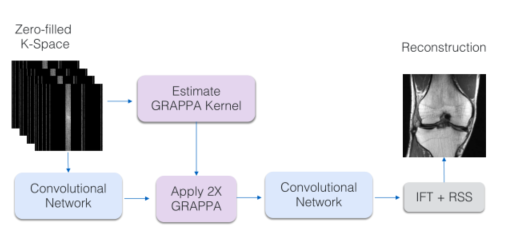
\includegraphics[scale=1]{./image/GRAPPANet.png}
	\caption{The GRAPPANet model}
	\label{GRAPPANet}
\end{figure}
<<<<<<< Updated upstream
\par 文\cite{hammernik2018learning}提出一种变分网络(Variatinal Network, VN),该方法将数学变分模型和深度神经网络相结合,将每一次的迭代重建与网络中的每一步骤相对应,即VN包含了数学优化模型中梯度下降的步骤。文\cite{LU2020106790}将pFISTA-SENSE的迭代过程作为ResNet的基本网络结构,提出了pFISTA-SENSE-ResNet模型,得到了比MoDL和VN质量更高的MRI重建图像。
\par 但是从目前来说,基于深度学习的方法仍未得到广泛应用,主要原因有:数据难以获取;训练得到的模型泛化能力不够强;当数据之间差异较大时,模型的重建结果质量较差;同时图像重建质量也容易到MRI设备参数的影响。
\cite{LI2021332}
=======
\par 基于深度学习的方法仍未得到广泛应用,主要原因有:由于病人隐私等问题的存在,MRI原始数据难以获取;训练得到的模型泛化能力不够强,当数据之间差异较大时,模型的重建结果质量较差;同时图像重建质量也容易到MRI设备参数的影响。更重要的是,使用深度学习进行MRI重建的方法与传统MRI重建方法相比,目前尚未体现其优越性,主要在重建图像质量和重建时间,并且还比较耗费资源用于训练模型。


>>>>>>> Stashed changes

\newpage
\bibliographystyle{IEEEtran}
\bibliography{reference}

\end{document}
